\documentclass[a4paper,11pt]{article}
\usepackage[dvips]{graphicx}
\usepackage[T1]{fontenc}
\usepackage[utf8]{inputenc}
\usepackage[french]{babel}
\usepackage{lmodern} \normalfont
\DeclareFontShape{T1}{lmr}{bx}{sc}{<-> ssub * cmr/bx/sc}{}
\usepackage{textcomp}
\usepackage{fixltx2e}
\usepackage{exptech} % inclusion du style immposé
\usepackage{amsmath}
\usepackage{amssymb}
\usepackage{graphicx}
\usepackage{wrapfig}
\usepackage{subcaption}
\usepackage{listings}
\usepackage{color}
\usepackage{pdfpages}
\usepackage[colorlinks=true,
			linkcolor=blue,
			bookmarksnumbered=true,
			pdftitle={Report},
			pdfauthor={Hoel K.},
			pdfborder={0 0 0},
			pdfsubject={mittelwerk}]{hyperref}

\title{\textbf{Contrôleurs dans l'espace}}
\author{Julien \textsc{Bouvet}, Antoine \textsc{Chenon}, Mikaïl \textsc{Demirdelen}, Hoel \textsc{Kervadec}
        \\
        Encadrants : Yann \textsc{Ricquebourg}, Loic \textsc{Helouet}}
\date{Juin 2014}
\markright{Contrôleurs dans l'espace}

\begin{document}
\thispagestyle{empty}

\maketitle
\begin{abstract}
    Parti d'un simulateur de vol spatial, nous avons créé une chaîne d'outils et un nouveau langage permettant de facilement automatiser les vaisseaux du dit simulateur, afin d'obtenir une vitrine technologique de la théorie du contrôle, et ainsi faciliter l'illustration de concepts plus abstraits.
\end{abstract}

\section{Présentation du Sujet}
    \subsection{Contexte}
        La théorie du contrôle a comme objet l'étude du comportement de systèmes dynamiques paramétrés en fonction des trajectoires de leurs paramètres. Elle sert à analyser les trajectoires de systèmes commandés.
				
				Cette théorie peut être utilisée de différentes manières : amener le système d'un état initial à un état final (l'objectif) ou assurer que le système ne se retrouve pas en mauvaise configuration...

    \subsection{Orbiter}
        Orbiter\footnote{http://orbit.medphys.ucl.ac.uk/} est un simulateur de vols spatiaux, développé par Dr. Martin Schweiger, qui était parti du constat que la simulation spatiale manquait cruellement d'un simulateur respectant les lois de la physique.

        \begin{figure}[!h]
            \begin{center}
                
\includegraphics[width=0.7\textwidth]{img/orbiter_logo.png}
            \end{center}
        \end{figure}

        La première version fut publiée le 27 novembre 2000, et la dernière version stable en date est la version 2010.

        Malgré le succès rencontré par le simulateur et les nombreuses demandes d'ouverture du code\footnote{D'un point de vue open source}, Mr. Schweiger a toujours refusé de le faire, et a préféré à la place sortir une API, afin tout de même de pouvoir laisser la possibilité de développer ses propres modules, vaisseaux, etc.

        Orbiter possède de base de nombreux vaisseaux, et un grand nombre de missions différentes, allant des missions historiques, aux plus futuristes. Cette grande variété en fait un outil idéal pour apprendre des concepts de la physique en s'amusant, et peut être une excellence base pour servir de démonstrateur.

    \subsection{La Théorie du contrôle}
        La Théorie du contrôle recoupe l'ensemble des disciplines qui consistent à asservir un système, et à lui permettre de s'auto gérer: c'est la base de l’auto pilotage.

        Un des principe les plus simples est la boucle de contrôle: en se basant sur plusieurs variables (puissance d'un réacteur, vitesse, altitude, ...), et en les comparants à des objectifs initiaux, nous pouvons adapter la puissance du réacteur, afin de minimiser l'écart entre réalité et théorie.

        \begin{figure}[!h]
            \begin{center}
                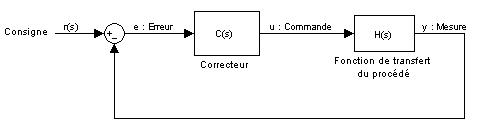
\includegraphics[width=1\textwidth]{img/boucle_controle.jpg}
                \caption{Exemple de système bouclé simple.}
            \end{center}
        \end{figure}

        Parti du constat que Orbiter est un outil ludique et visuel, il a été proposé de créer une chaîne d'outils permettant d'automatiser facilement des vaisseaux d'Orbiter à l'aide de boucles de contrôles.

    \subsection{Objectifs initiaux}
        Pour automatiser les vaisseaux, nous avons été chargé de créer un nouveau langage, à la grammaire épurée, laissant place à des fonctions basiques, et pouvant ainsi servir facilement de démonstrateur pour la théorie du contrôle.

        Nous pourrions par exemple, nous en servir lors d'expositions ou de conférences à missions de vulgarisation, pour montrer facilement les différentes manières d'aborder l'asservissement d'un vaisseaux.

        Le langage devait donc être très simple, et la chaîne logicielle la plus simple possible à utiliser, pouvant permettre à quiconque de créer ses propres automates.

        Par ailleurs, le travail devait être réutilisable, pour pouvoir être reprit les années suivantes, et ainsi améliorer petit à petit ce compilateur.

\section{Réalisation pratique}
    \subsection{Déroulement des opérations}
        Notre travail s'est porté sur un seul vaisseaux (le ShuttleA), afin de nous concentrer sur la grammaire et notre compilateur. C'est aussi dû au fait que le Shuttle A est un vaisseau composé d'une seule classe C++, ce qui permet une intégration plus simple de notre automate. Une amélioration du projet pourrait être de supporter un plus grand nombre de vaisseaux (voir tous?) une fois que le langage est jugé suffisamment mature.
				
				\begin{figure}[!h]
            \begin{center}
                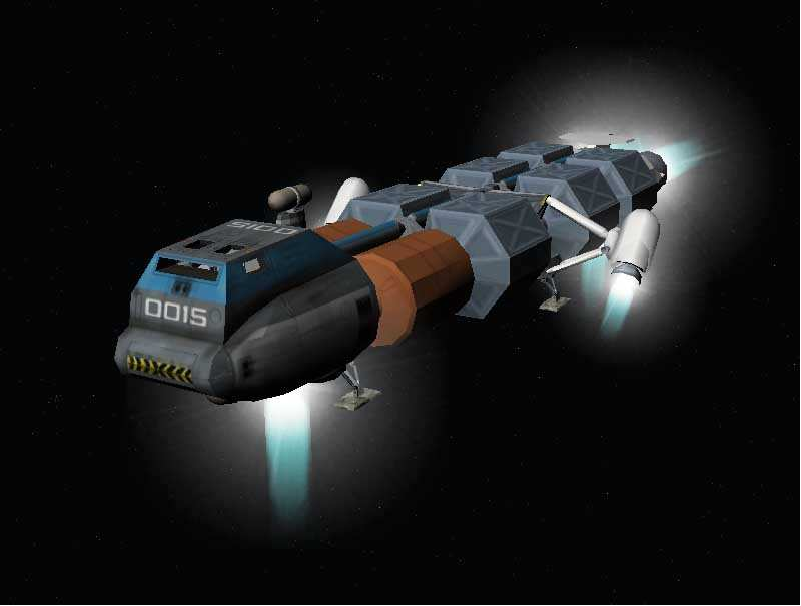
\includegraphics[width=1\textwidth]{img/shuttleA.png}
                \caption{Le Shuttle A}
            \end{center}
        \end{figure}
				

    \subsubsection{Recompilation des vaisseaux existants}
        Nous avons utilisés Orbiter 2010 et son sdk, afin de pouvoir dans un premier temps recompiler les vaisseaux du simulateur, sans les altérer.

        Nous avons dû utiliser Visual Studio\footnote{Nous avons accès à la version Pro 2013 grâce à Dreamspark, la plate forme de Microsoft.}, puisque le code des vaisseaux est livré sous forme de projet Visual Studio. Cette dépendance à Visual studio nous empêche de créer une chaine logicielle propre, et légère\footnote{Une installation de visual studio peut faire plusieurs giga octets.}.

        Voulant nous concentrer sur la langage, il a été décidé de continuer avec cette dépendance, pour potentiellement la supprimer plus tard.
				
				\begin{figure}[!h]
            \begin{center}
                
\includegraphics[width=1\textwidth]{img/visual-studio-logo.jpg}
                \caption{Visual Studio}
            \end{center}
        \end{figure}

    \subsubsection{Première automatisation}
        Une fois le vaisseaux compilé et utilisable, nous avons pu éditer directement son code c++, afin de comprendre le fonctionnement de celui ci, et surtout de l'API\footnote{Application Programming Interface} d'Orbiter.

        Après quelques essais, nous avons réussi à former un "pattern", qui pourrait être produit par un compilateur.

    \subsubsection{Javacc, le retour de la vengeance}
        Ayant réalisé en parallèle de l'étude pratique un projet compilateur, il nous a semblé naturel de réutiliser les mêmes outils, à savoir, Javacc. Cela nous a permis de gagner un temps précieux sur la prise en main de l'outil principal de développement.

        Javacc est un compilateur de compilateur, permettant de facilement créer un analyseur syntaxique, et de construire à partir de lui un analyseur sémantique et bien entendu, notre compilateur.
				
				\begin{figure}[!h]
            \begin{center}
                
\includegraphics[width=100pt]{img/java.png}
                \caption{Java}
            \end{center}
        \end{figure}

    \subsubsection{Le langage}
        L'objectif était de garder un langage simple, avec des fonctionnalités limités: pas de tableaux, pointeurs, et autres.

        Même si ce choix peut paraître étrange, on peut argumenter que complexifier le langage lui ferait perdre son intérêt\footnote{Rappelons qu'il s'agit d'un langage de démonstration, qui doit pouvoir être pris en main par des personnes n'ayant jamais programmé ou presque}, puisqu'il suffirait d'apprendre directement le c++ et ne plus être limité par notre langage.
        
        Ci dessous la grammaire presque complète (certaines parties étant suffisamment explicites, nous ne les détailleront pas).

        \begin{align}
            Automata &= VesselName()\nonumber\\
                &~~~~ThrusterDeclaration()*\nonumber\\
                &~~~~FunctionDeclaration()~\nonumber\\
                &~~~~StateDeclaration()~\nonumber\\
                &~~~~EOF\nonumber\\
            VesselName &= <ident>\nonumber\\
            ThrusterDeclaration &=  ~<ident> ":" <ident>\nonumber\\
            FunctionDeclaration &=  ~Type() <ident> "(" Args() ")" "\{"\nonumber\\
                &~~~~ Instruction()* \nonumber\\ 
                &~~~~ "\}" \nonumber\\ 
            StateDeclaration &=  ~<ident> "\{"\nonumber\\
                &~~~~ Instruction()* \nonumber\\
                &~~~~ "\}" \nonumber\\
            Instruction &= DeclVar()\nonumber\\
                &~~~~|~Affect()\nonumber\\
                &~~~~|~If() \nonumber\\
                &~~~~|~While() \nonumber\\
                &~~~~|~Return()\nonumber\\
                &~~~~|~Gotogoto() \nonumber\\
                &~~~~|~ApiGet() \nonumber\\
            Gotogoto() &= "GOTOGOTO" <ident>\nonumber\\
            ApiGet&= "API\_GET"~"\{" \nonumber\\
                &~~~~ Getter()*\nonumber\\
                &~~~~ "\}"\nonumber\\
           Getter &=  Dests()~"="~<ident>~"("~Args()~")"~";"\nonumber\\
            Dests &=  <ident> (( "," <ident>)*)?\nonumber\\
        \end{align}

        Cette grammaire a été gardée au plus simple (on aurait pu par exemple interdire les return directement dans la grammaire), et ne suffit pas à interdire tout les abus de l'utilisateur. Ce travail est laissé à l'analyseur sémantique, qui s'assure de la cohérence et la validité des opérations demandées.
        
        On peut remarquer l'étrangeté d'ApiGet. Il s'agit d'une conséquence d'un choix technique, qui visait à rendre la récupération des informations sur le vaisseaux simple. 
        
        Par exemple, lorsque l'on récupère la vitesse du vaisseaux, on va récupérer au total 3 doubles: la vitesse en x, y, et z. Nous avons donc voulu obtenir une syntaxe du type \[ x,y,z = GET\_SPEED(); \], ce qui entrait en conflit avec les affectations habituelles\footnote{Une amélioration possible (mais difficile techniquement à mettre en place) pourrait être la généralisation du renvois multiple, par exemple avec la création d'un type tuple.}.



    \subsection{Objectifs atteints}
        Nous avons un langage de défini, et un compilateur qui fonctionne permettant de produire du code c++ valide.

    \subsection{Améliorations possibles}
        Plusieurs améliorations sont possibles à l'avenir, et peuvent constituer suffisamment de travail pour potentiellement en faire un nouveau sujet d'étude pratique pour les années futures.
        On peut lister (du plus important au moins important):
        \begin{itemize}
            \item Supprimer la dépendance à Visual Studio, pour avoir une vrai chaine logicielle
            \item Avoir un plus grand nombre de vérifications lors de la compilation. Dans l'absolu, si le compilateur c++ produit une erreur (ou un warning), le compilateur devra avoir affiché une erreur/warning en premier lieu.
            \item Supporter un plus grand nombre de vaisseaux, en retravaillant un peu la grammaire et l'intégration du code.
						\item Trouver de nouveaux automates pour les démonstrations lors d'expositions ou de conférences 
						\item Ajouter une GUI permettant de choisir son vaisseau et son automate
        \end{itemize}

\section{Conclusion}
    Bien que les principaux objectifs aient été atteint, des finitions sont toujours souhaitable.

    On peut tout de même noter qu'il s'agit d'un projet intéressant, puisque touchant à plusieurs domaines à la fois, suffisamment pour continuer le travail dessus, afin de produire à terme une véritable vitrine de démonstration pour la théorie du contrôle.
		
		Travailler sur ce simulateur nous a vraiment plus. Quelle fierté lorsque notre Shuttle A a fini par s'élever tout seul. 
		Ce projet permet de croiser un domaine très théorique (la théorie du contrôle) avec quelque chose de concret (une fusée qui décolle). C'est cela qui rend ce projet valorisant et passionnant.


%\bibliography{biblio} % inclusion de biblio.bib

\end{document}
